\section{Misura di alcune resistenze}
\paragraph{Montaggio del circuito con resistenza R e acquisizione dati\\}
Per prima cosa abbiamo ordinato le resistenze controllando le barre colorate che ne codificano  i valori nominali e, utilizzando il multimetro digitale, abbiamo misurato il valore esatto di resistenza. Come ci si aspettava, tali valori erano compatibili con i valori nominali entro l'incertezza fornita dal costruttore.

Per montare il circuito abbiamo sfruttato le bocchette della breadboard a nostra disposizione e alcuni cavi supplementari per assicurarci un buon contatto tra le varie parti del circuito.
Sapendo che vi era necessità di cambiare spesso configurazione tra ``amperometro a monte'' e ``amperometro a valle'', abbiamo inizialmente costruito un circuito di una sola maglia comprendente il generatore di ddp, l'amperometro e la resistenza da misurare. 
%Si è passati dunque a montare il circuito. Ricordiamo che sono state sfruttate le bocchette della breadboard per collegare la resistenza al circuito. Così facendo, è stato assicurato un buon contatto con i cavi principali (evitando così che accidentalmente potesse staccarsi nel momento in cui trafficavamo con il cablaggio).
Solo allora abbiamo aggiunto il voltmetro in modo tale che bastasse spostare un solo contatto per cambiare la posizione circuitale dell'amperometro. In Fig. \ref{fig:circuiti} sono riportati gli schemi circuitali delle due configurazioni.

Prima di procedere all'acquisizione dati, abbiamo calcolato il valore massimo di tensione applicabile al circuito. Infatti, 2 delle resistenze da noi utilizzate potevano dissipare una potenza massima di $0.25\si{\watt}$  ($100 \si{\kilo\ohm}$ e $1\si{\ohm}$) mentre le rimanenti di $0.5\si{\watt}$ . Utilizzando la legge di Joule, $P=\frac{V^2}{R}$ e invertendola, abbiamo ottenuto la $V_{MAX}$ applicabile. % avevi scritto 0.5W per entrambe le resistenze, qual è il valore corretto?

Abbiamo dunque chiuso il circuito e annotati i valori di tensione e corrente forniti dai due tester ICE. Ricordiamo che per evitare di rovinare i delicati strumenti abbiamo sempre lasciato il tester usato per misurare correnti sulla scala $5A$, cambiando poi scala progressivamente facendo attenzione a non uscire dal $range$. È importante notare che l'incertezza sul valore letto è $\frac{1}{50}$ del fondo-scala utilizzato. Per questo motivo si è sempre cercato di mantenere la lancetta degli strumenti oltre la metà del quadrante graduato anche se non sempre è stato possibile ottenere tale situazione per entrambi i tester.

 Abbiamo inoltre provato a valutare l'errore statistico su una singola misura aprendo e chiudendo il circuito. Si è subito visto che il valore riportato dagli strumenti rimaneva invariato, indice che la precisione dello strumento non ci permetteva di apprezzare l'errore statistico.

\paragraph{Analisi dati\\}

Abbiamo inizialmente calcolato il valore delle resistenze applicando l'equazione $R_m=\frac{V_m}{I_m}$. Si è notata subito una notevole differenza con i valori misurati dal multimetro digitale per i valori di resistenza $1 \Omega$ e $1M \Omega$. Tale discrepanza è dovuta alle resistenze interne del voltmetro e dell'amperometro che ne disturbano la misura. Questo problema è stato risolto considerando il circuito con gli strumenti di misura non ideali. Dunque, utilizzando le equazioni di Kirchhoff, abbiamo calcolato i valori di $R_X$ in funzione delle resistenze interne degli strumenti di misura e dei valori di corrente e tensione misurati. Le relazioni da noi ottenute sono:\\
\\
\noindent\begin{minipage}{.5\linewidth}
\begin{equation}
R_X=\frac{R_VV}{V-IR_V}
\label{casapagliaccio}
\end{equation}
\end{minipage}%
\begin{minipage}{.5\linewidth}
\begin{equation}
R_X=\frac{V}{I}-R_A
\label{brugnagay}
\end{equation}
\end{minipage}
\break
dove l'equazione (\ref{casapagliaccio}) è riferita al circuito (a) mentre l'equazione (\ref{brugnagay}) è relativa a (b). Abbiamo indicato con $R_V$ e $R_A$ le resistenze interne degli strumenti utilizzati. 
Ricordiamo che per calcolare i valori $R_V$ e $R_A$ sono stati risolti i circuiti interni degli strumenti stessi, forniti dal produttore. 

Riportiamo ora il grafico delle resistenze, misurate tramite multimetro digitale e tester ICE\footnote{Per il calcolo delle incertezze sulle misure derivate abbiamo utilizzato le usuali leggi di propagazione degli errori.}. 

\begin{figure}[h]
    \centering
        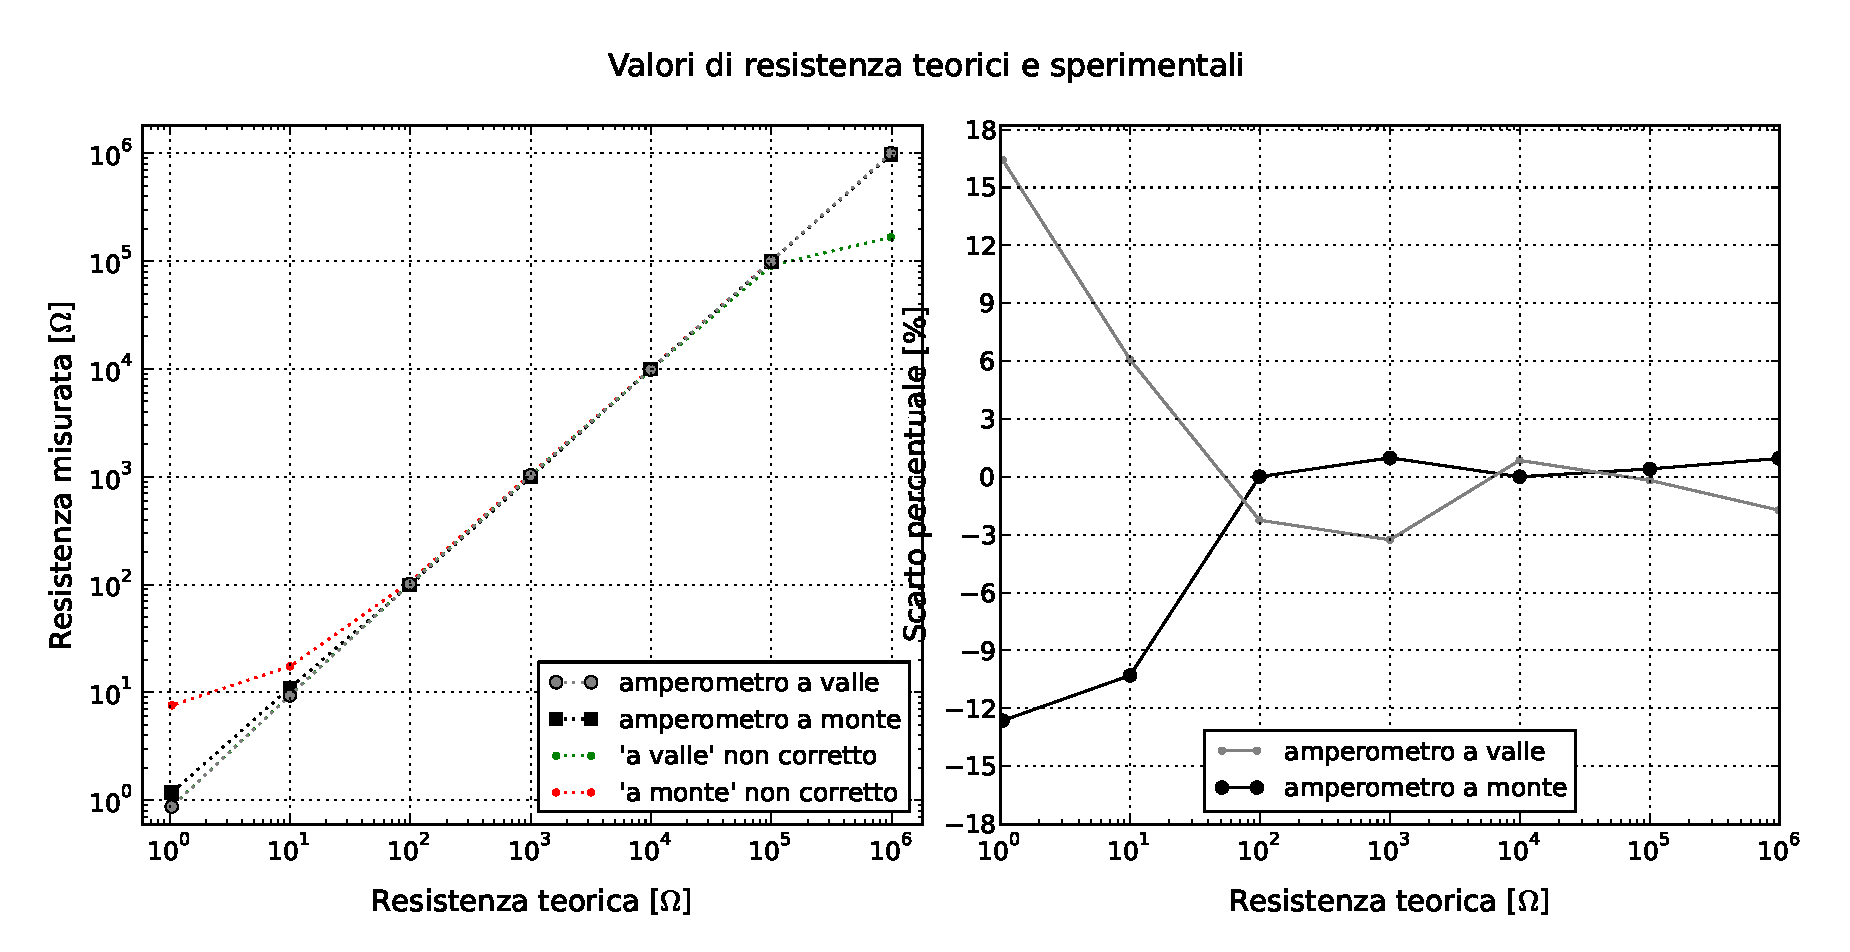
\includegraphics[width=\textwidth]{Res.eps}%{Res_70.eps}
        \caption{Il primo grafico mostra i valori sperimentali delle resistenze, sia corretti con le resistenze interne degli strumenti di misura che senza tale correzione, in funzione dei valori teorici delle resistenze. Si noti che il grafico ha entrambi gli assi in scala logaritmica. Il secondo grafico mostra invece gli scarti in percentuale tra il valore sperimentale delle resistenze e quello teorico. In questo grafico solo la scala sull'asse delle ascisse è logaritmica.}
        \label{fig:resistenze}
\end{figure}

\paragraph{Considerazioni\\}
In Figura (\ref{fig:resistenze}) si nota che per resistenze piccole ($\approx$ 1 $\Omega$) la misura effettuata con il circuito ``a valle'' risulta essere, se non si applicano correzioni, non compatibile con il valore reale di resistenza. È facile capire il motivo di ciò analizzando il circuito: ricordando l'equazione (\ref{brugnagay}), vediamo subito che $\frac{V}{I}=R_X+R_A$. Dunque, se $R_A$ ed $R_X$ sono confrontabili tra loro, è evidente che il valore stimato sarà completamente sbagliato. Analogamente, si vede che il circuito ``a monte'' non fornisce un valore attendibile di $R_X$ per resistenze grandi ($\approx$ 1 $M\Omega$). Infatti dall'equazione (\ref{casapagliaccio}) si deduce che l'amperometro sentirà una resistenza a valle pari a $R_{eq}=(\frac{1}{R_V}+\frac{1}{R_X})^{-1}$. È evidente che, nel momento in cui $R_X \approx R_V$ e addirittura $R_X > R_V$, la resistenza del tratto circuitale comprendente voltmetro e resistenza in esame sarà minore di $R_X$.

Per valori di resistenza intermedi ($1000-100000 \Omega$) entrambi i circuiti si dimostrano validi e anche senza applicare correzioni si può ottenere una buona stima di $R_X$.

Infine, applicando la correzione abbiamo notato che non vi sono differenze apprezzabili tra i due circuiti utilizzati per ricavare il valore incognito di resistenza. È possibile ottenere con ambedue i sistemi un valore di $R_X$ affetto da errore percentuale anche solo del $2\%$ nei casi migliori. Ricordiamo infatti che i dati affetti da errori percentuali più grandi sono quelli in cui non siamo riusciti ad ottimizzare il fondo scala (vedi Fig. \ref{fig:circuiti}, per $1\si{\ohm}$ e $10\si{\ohm}$ non siamo infatti riusciti a tenere gli indicatori di entrambi strumenti oltre la metà quadrante). %Potrebbe essere interessante notare che il valore misurato con amperometro ``a monte'' per la resistenza di 1 $M \Omega$ risulta affetto da un errore percentuale consistente. Durante l'esperienza abbiamo effettuato questa misura con una tensione di 7 V, mentre la relativa misura ``a valle'' con tensione di 40 V. Non possiamo dire con certezza che causa di tale errore sia la diversa tensione applicata ma, visto che per le altre resistenze abbiamo tenuto praticamente invariata la tensione eseguendo le misure "monte" e "valle" e per ciascuna coppia gli errori sono circa uguali con entrambi i metodi, ciò potrebbe essere indice che lo strumento funziona in modo più preciso quando sia tensione che corrente che scorre nel circuito sono più alte. ***CREDO SIA UNA CAZZATA QUESTA, E' COLPA DEL FONDOSCALA DI MMIERDA***
